\section{Evaluation}\label{sec:evaluation}
The result of strong and weak scaling studies of the vectorized code is shown in Figure \figref{strong scaling} and Figure \figref{weak scaling}. In the strong scaling study, we examined the time spent with varies frame sizes while keeping the number of threads constant; in our case. we used 24 threads. The result shows that the time spent increases linearly as we increase the frame size. In the weak scaling study, we tested the time spent using varies number of thread while keeping the frame size 4000. The time spent decreases in log scale as we increase the number of thread. 

\begin{figure}[h]
	\centering
	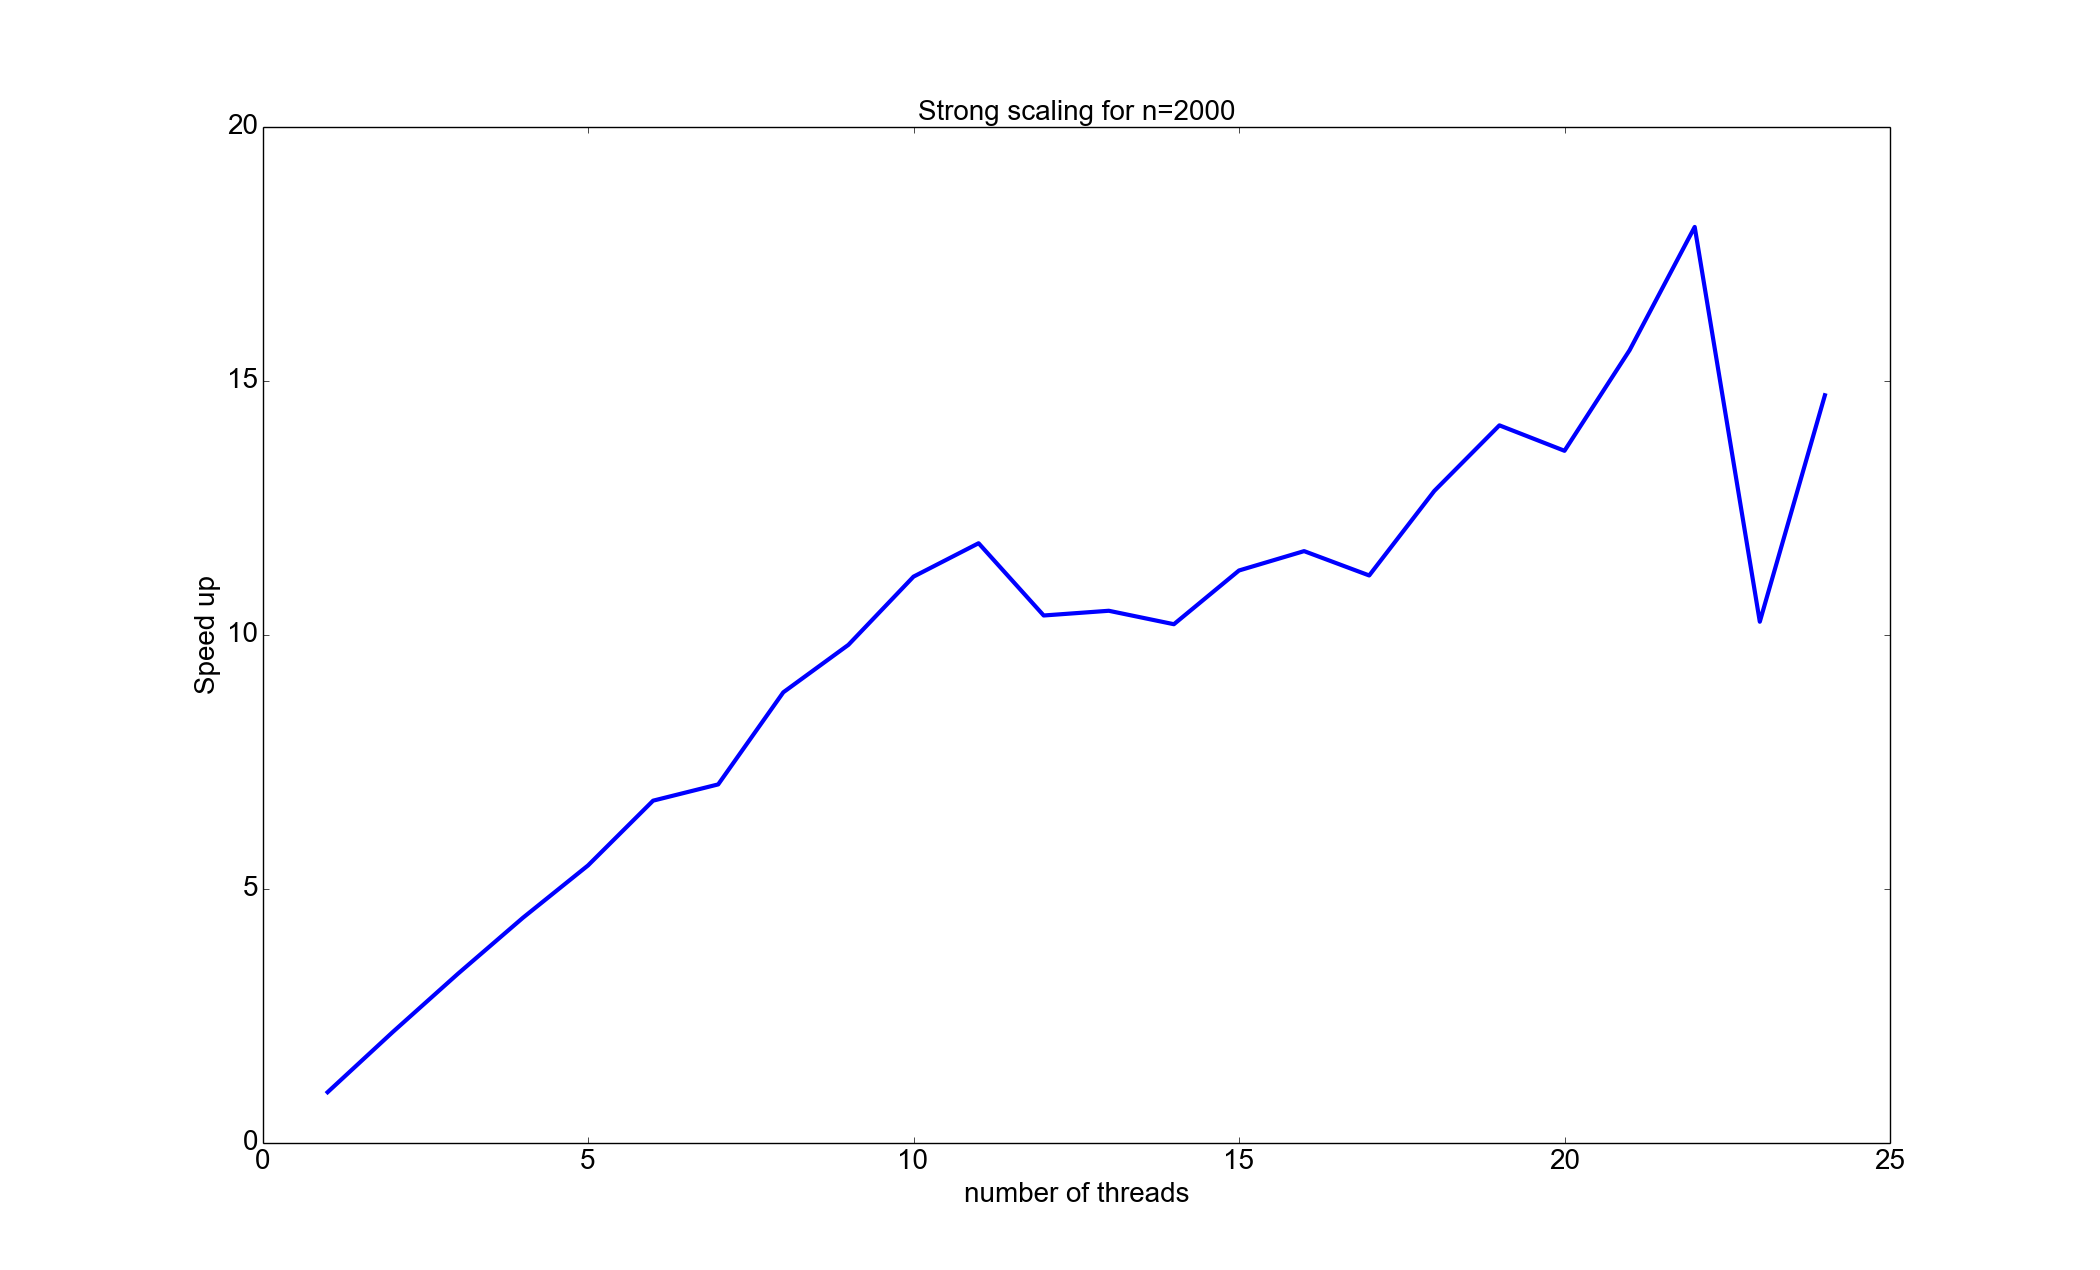
\includegraphics[width=0.8\textwidth]{figs/strong_scaling.pdf}
	\caption{Strong scaling study with 24 threads and varies number of frames}
	\label{fig:strong scaling}
\end{figure}


\begin{figure}[h]
	\centering
	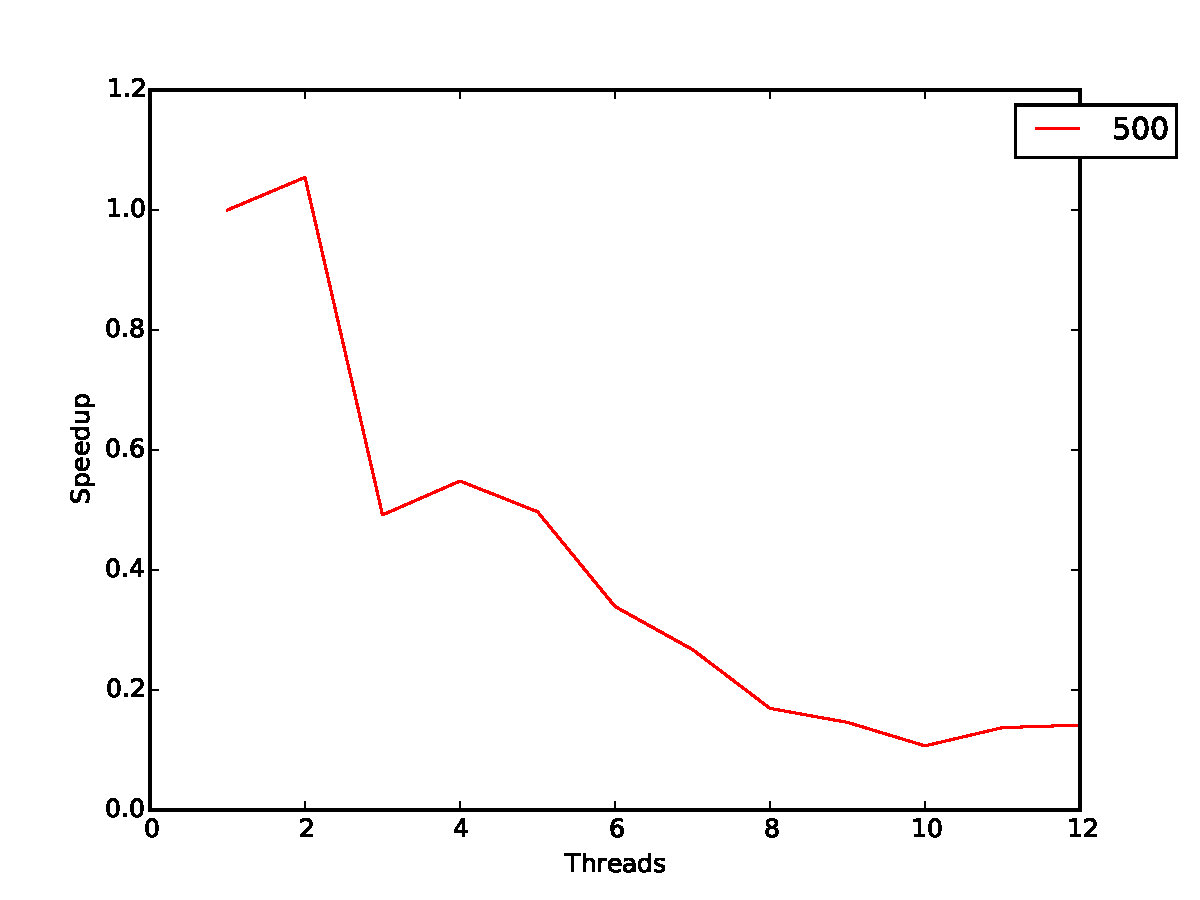
\includegraphics[width=0.8\textwidth]{figs/weak_scaling.pdf}
	\caption{Weak scaling study with frame size 4000 and varies number of threads}
	\label{fig:weak scaling}
\end{figure}
